\documentclass[11pt,twocolumn]{article}

\usepackage[preprint]{acl}
\usepackage{times}
\usepackage{latexsym}
\usepackage[T1]{fontenc}
\usepackage[utf8]{inputenc}
\usepackage{microtype}
\usepackage{graphicx}
\graphicspath{{figures/}}
\usepackage{booktabs}
\usepackage{amsmath}
\usepackage{multirow}
\usepackage{xcolor}
\usepackage{subcaption}

% Tighten float spacing to prevent page overflow
\setlength{\textfloatsep}{12pt plus 1.0pt minus 2.0pt}
\setlength{\floatsep}{12pt plus 1.0pt minus 2.0pt}
\setlength{\intextsep}{12pt plus 1.0pt minus 2.0pt}
\setlength{\dbltextfloatsep}{12pt plus 1.0pt minus 2.0pt}
\setlength{\dblfloatsep}{12pt plus 1.0pt minus 2.0pt}

\title{ExpenseSense: Privacy-Preserving On-Device Personal Finance Tool Calling with Sub-2B LLMs}

\author{Sajag Swami \qquad Yash Pandey \\
  Independent Researchers \\
  \texttt{sajagswami@gmail.com} \qquad \texttt{ya.pandey@outlook.com}}

\begin{document}
\maketitle

\begin{abstract}
Personal finance data - detailed records of when, where, and how a user spends money - is among the most sensitive information individuals possess, making cloud-based LLM inference undesirable for many users.
Yet natural-language personal finance assistants currently require transmitting these queries to cloud-hosted
LLMs, exposing users to data retention and third-party data flows.
We introduce \textbf{ExpenseSense}, a personal finance Q\&A assistant that runs entirely on-device, ensuring that no financial
records, query text, or model outputs leave the user's device.
To evaluate whether this privacy architecture is practically viable,
we benchmark on-device tool calling using a 115-question test suite
across six sub-2B quantized SLMs (0.8B-2B), comparing single-agent
(joint routing and parameter extraction) against dual-agent
(router-specialist) architectures.
The dual-agent advantage is metric-specific:
while optimised single-agent Qwen3.5-2B reaches the highest Task
Accuracy (92.0\%), dual-agent Qwen3.5-2B achieves 77.6\% strict
Correct Ratio (+17.4~pp over single-agent) while reducing average
latency by 48\%, and dual-agent Qwen3.5-0.8B reaches 89.1\% Task
Accuracy in 3.0~s with 1.2\,GB RAM.
Critically, dual-agent architectures shift errors from spurious
parameters to safer, missing parameters, reducing the risk of silent
incorrect outputs.
Our results demonstrate that private, high-quality financial analytics
is achievable on consumer hardware today, with no cloud dependency.
\end{abstract}

% ─────────────────────────────────────────────────────────────────────────────
\section{Introduction}
% ─────────────────────────────────────────────────────────────────────────────

Large language models (LLMs) have rapidly advanced tool-augmented AI
\citep{schick2024toolformer, patil2023gorilla, qin2023toolllm},
enabling agents to invoke structured APIs from natural language.
However, research primarily targets large cloud-hosted models which
is problematic for personal finance where local inference is necessary
for privacy.
Expense records reveal sensitive behavioral patterns (e.g., health-related purchases). 
Users expect natural language interfaces (e.g., asking ``how much did I spend on
food last month?'') that map to structured queries over local data
\citep{li2024personal}.
This creates an underexplored problem: can \emph{sub-2B quantized
models} running entirely on consumer hardware reliably call
domain-specific financial tools from informal, colloquial language,
and in doing so, serve as practical privacy infrastructure for real
users?

Existing benchmarks \citep{qin2023toolllm,
finmcpbench2026, fintrace2026} focus primarily on multi-step trajectories across financial APIs for cloud-scale models,
which are prohibitively slow for local deployment.
Conversely, on-device models like Octopus~v2 \citep{chen2024octopus}
and Hammer \citep{lin2024hammer} demonstrate the potential of smaller
models but have not been evaluated on domain-specific financial
schemas or under consumer-hardware latency constraints.

We address three research questions (\textbf{RQ}):

\begin{itemize}\itemsep=0pt \parskip=0pt \parsep=0pt
  \item \textbf{RQ1}: Does on-device inference with sub-2B SLMs
        provide a practically viable privacy protection for personal
        finance tool use-i.e., can users obtain accurate financial
        analytics without surrendering query data to cloud providers?
  \item \textbf{RQ2}: Does decomposing intent classification from
        parameter extraction (dual-agent) yield significant accuracy
        gains over a joint single-agent architecture?
  \item \textbf{RQ3}: What are the primary failure modes across
        architectures, and do they differ in the human-facing harms
        they produce?
\end{itemize}

This paper introduces \textbf{ExpenseSense}, with the following
contributions:

\begin{enumerate}
    \item Empirical \textbf{on-device deployment guidelines for
          privacy}: Demonstrating that sub-2B SLMs on consumer hardware
          (e.g., Qwen3.5-0.8B in dual mode achieving 89.1\% Task Accuracy
          in 3.0~s with 1.2\,GB RAM) provide a practical privacy protection,
          eliminating cloud data transmission for personal finance.

    \item A comparative \textbf{architectural evaluation} of single- vs.\
          dual-agent setups across six sub-2B models using a \textbf{7-feature
          complexity scoring model} (L1--L3 tiers) to systematically benchmark
          performance under realistic, informal query constraints.

    \item A fine-grained \textbf{error taxonomy} of 7 categories showing
          that dual-agent decomposition consolidates errors into safer, predictable
          failure modes---shifting from dangerous spurious parameter additions
          (\texttt{PARAM\_EXTRA}) toward visible omissions (\texttt{PARAM\_MISSING}).
\end{enumerate}

% ─────────────────────────────────────────────────────────────────────────────
\section{On-Device Inference as Privacy Protection for Real Users}
\label{sec:privacy}
% ─────────────────────────────────────────────────────────────────────────────

The deployment of LLMs in personal finance exposes a structural
tension: the same conversational interface that makes financial
analytics accessible to users also makes their sensitive
behavioral data accessible to cloud providers.
When a user types "how much did I spend on therapy last month?" into
a cloud-hosted assistant, they are not merely querying a
database-they transmit evidence of a health condition, a temporal 
pattern, and financial commitment to a third-party infrastructure 
they did not choose and cannot audit. The query is a disclosure.

\citet{staab2024memorization} demonstrated that LLMs can infer
sensitive personal attributes-including location, income, and
demographic characteristics-from seemingly innocuous texts, and
\citet{yao2024survey} catalog privacy risks including data leakage,
memorization, and inference attacks.
The implication for personal financial assistants is direct: even if the
database never leaves the device, routing natural-language queries
through cloud LLMs leaks behavioral signals that can be retained,
aggregated, and exploited beyond the user's control or knowledge.

ExpenseSense addresses this threat by adopting an \emph{on-device,
privacy-first} architecture.
By leveraging sub-2B quantized models that run efficiently on consumer
hardware (tested on an Apple M1 with 8\,GB unified memory), all user
data, query text, and model outputs remain strictly local.
No financial records, queries or inferences leave the device.

The local-first design preserves \emph{contextual integrity}
\citep{nissenbaum2004privacy} by ensuring financial queries and data
remain within their original context.

The practical threat model covers three risks: cloud data retention, query-level
inference attacks \citep{staab2024memorization}, and third-party exposure.
On-device inference eliminates all three by ensuring queries never
leave for external infrastructure.

The key challenge is that on-device inference with sub-2B models has
historically been unreliable for structured tool calling
\citep{kavathekar2025small}.
Our work demonstrates that architectural decomposition-separating
intent classification from parameter extraction-bridges this
reliability gap, making private on-device inference not merely
possible but practical.

% ─────────────────────────────────────────────────────────────────────────────
\section{Related Work}
% ─────────────────────────────────────────────────────────────────────────────

\paragraph{Tool-Augmented Language Models.}
Toolformer \citep{schick2024toolformer} demonstrated self-supervised
tool-use learning; Gorilla \citep{patil2023gorilla} and ToolLLM
\citep{qin2023toolllm} scaled to thousands of real-world APIs.
HuggingGPT \citep{shen2024hugginggpt} and ToolAlpaca
\citep{tang2024toolalpaca} explored multi-step orchestration.
APIGen \citep{liu2024apigen} introduced a verified pipeline for
generating function-calling training data, showcasing that 1B-parameter
models fine-tuned on high-quality synthetic data can surpass
GPT-3.5-Turbo on structured tool invocation.
These approaches rely on cloud-hosted models ($\ge$7B), leaving the
privacy-constrained on-device setting largely unaddressed.

\paragraph{Function-Calling Evaluation.}
The Berkeley Function Calling Leaderboard \citep{yan2024bfcl}
established a benchmark using AST substring matching and
execution-based validation.
\citet{kavathekar2025small} proposed an evaluation suite (FSP, ACS,
AVC, Task Accuracy, and Correct Ratio) to evaluate small model
function calling; we adopt these metrics
directly.
CallNavi \citep{callnavi2025} proposed a two-stage router+specialist
approach-similar to our dual-agent design-but evaluates models
$\geq$7B on general-purpose APIs.
In contrast, we focus on sub-2B models for domain-specific,
single-turn personal finance related tasks.

\paragraph{On-Device Function Calling.}
MobileLLM \citep{liu2024mobilellm}, Phi-3 \citep{abdin2024phi3}, and
related surveys \citep{xu2024ondevice} have explored sub 4B parameter
models for mobile deployment.
Octopus~v2 \citep{chen2024octopus} fine-tuned a 2B model for
on-device API calling via functional tokens, achieving competitive
latency against GPT-4 on specific tasks.
Hammer \citep{lin2024hammer} introduced function masking to reduce
overfitting to function names, addressing an issue similar to the
category normalisation errors we observe.
Apple Intelligence \citep{gunter2024apple} validated on-device tool
calling at scale with a $\sim$3B model, demonstrating the viability
of the paradigm.
\citet{kavathekar2025small} found that structured output compliance is
the primary bottleneck for SLMs.

\paragraph{Financial NLP and Privacy.}
FinQA \citep{chen2022finqa} and FinGPT \citep{yang2023fingpt} target
financial numerical reasoning and generation, but focus on text
generation rather than tool calling.
FinMCP-Bench \citep{finmcpbench2026} and FinTrace \citep{fintrace2026}
evaluate LLM agents for financial tool use, focusing primarily on multi-step,
long-horizon trajectories across cloud-scale models.
Personal finance assistants \citep{li2024personal} require strict
privacy, making local execution crucial.

\paragraph{Human-Centered Privacy for Language Models.}
A growing body of work has seen privacy not as a technical property of
models but as a human-centered concern shaped by user expectations and
social context.
\citet{nissenbaum2004privacy}'s contextual integrity framework can be 
applied to conversational AI to show that data flows violate
privacy when they cross contextual norms, even when no explicit PII is
transmitted.
\citet{staab2024memorization} demonstrated that LLMs act as inference
engines, reconstructing sensitive personal attributes from ordinary
text- a threat particularly acute when personal finance queries are routed
through cloud providers.
\citet{yao2024survey} surveys the resulting landscape of data
leakage, memorization, and inference risks in deployed LLM systems.
Our work operationalises these concerns at the system level: rather
than studying how cloud LLMs violate privacy, we build and evaluate an
architecture that eliminates the exposure pathway entirely, keeping
all query data local to the user's device.

% ─────────────────────────────────────────────────────────────────────────────
\section{System Design}
% ─────────────────────────────────────────────────────────────────────────────

\subsection{Tool Inventory}

ExpenseSense exposes five analytical tools over a user's expense
database.
Table~\ref{tab:tools} summarises each tool and its parameter space.
These tools span core personal finance use cases: time series
analysis, categorical breakdown, period comparison, aggregation, and ranked retrieval.

\begin{table}[t]
\centering
\small
\resizebox{\columnwidth}{!}{%
\begin{tabular}{@{}p{3.9cm}cp{4.0cm}@{}}
\toprule
\textbf{Tool} & \textbf{ID} & \textbf{Key Params} \\
\midrule
\texttt{plot\_time\_series}     & 1 & category, year/month, ranges, months, ignore\_rent \\
\texttt{plot\_distribution}     & 2 & category, year/month/day, ranges, months, ignore\_rent \\
\texttt{plot\_comparison\_bars} & 3 & category, y1/m1, y2/m2, sm/em/ey, ignore\_rent \\
\texttt{calculate\_total}       & 4 & category, remarks, year/month/day, months, ignore\_rent \\
\texttt{get\_top\_expenses}     & 5 & n, category, year/month/day, months, min\_amount, ignore\_rent \\
\bottomrule
\end{tabular}%
}
\caption{Tool inventory. The five tools span visualisation (1--3),
aggregation (4), and retrieval (5).}
\label{tab:tools}
\end{table}

\subsection{Architectural Configurations}

We evaluate two local architectures for mapping natural language user
queries to tool calls.

\paragraph{Single-Agent Pipeline.}
The single-agent pipeline uses a single prompt with all five tool
definitions, parameter schemas, and joint few-shot examples.
The model must select the tool and extract parameters in a single
pass, outputting a JSON object containing the tool ID (1--5) and
arguments for the chosen tool.
The prompt includes structured output rules, date-handling
instructions, and 73 tool-specific examples aggregated across all 5
tools.
Prompt length: $\approx$5,500 tokens (context window inclusive).

\paragraph{Dual-Agent Pipeline.}
The task is decomposed into two sequential inference calls:
\begin{enumerate}
    \item \textbf{Router}: A focused intent-classification prompt
          with 19 few-shot examples and explicit disambiguation rules
          (e.g., ``compare'' requires two distinct time periods) elicits
          a single digit (1--5).
    \item \textbf{Specialist}: The predicted tool ID selects a
          tool-specific prompt containing 13--16 examples for that
          \emph{one} tool, along with detailed parameter definitions
          and date-handling rules.
\end{enumerate}
The router sees $\approx$1,000 tokens; the specialist sees
$\approx$1,500--2,000 tokens with deeper, more directly relevant
supervision.
This simplifies the task for each model call and provides more
relevant in-context examples, though it requires two sequential
inference passes.
Combined prompt tokens: $\approx$2,700 per query.

\subsection{Post-Hoc Parameter Validation}
\label{sec:validation}

A post-processing validation layer corrects category names
deterministically without additional model calls:

\begin{enumerate}
    \item \textbf{Exact match} against the known vocabulary.
    \item \textbf{Morphological normalisation}:
          \texttt{groceries}$\to$\texttt{grocery},
          \texttt{caf\'{e}s}$\to$\texttt{cafe}.
    \item \textbf{Edit-distance matching} via difflib
          (cutoff $\geq 0.80$).
    \item \textbf{Token overlap scoring} (Jaccard;
          cutoff $\geq 0.50$).
\end{enumerate}

All results report both raw (pre-validation) and validated
(post-validation) metrics.

% ─────────────────────────────────────────────────────────────────────────────
\section{Benchmark Design}
\label{sec:benchmark}
% ─────────────────────────────────────────────────────────────────────────────

\subsection{Test Suite}

The benchmark contains 115 test cases across five task groups
(Table~\ref{tab:tc_distribution}).
Queries are written in natural and informal language: abbreviations
(\emph{``compare electricity '24 vs '25''}), colloquialisms
(\emph{``can ya tell me''}), misspellings (\emph{``distribuution''}),
and domain-specific terms (\emph{``combinis''}, \emph{``nomikais''},
\emph{``shinkansen''}).
This mimics the Japan-based personal finance context of the target
application and tests robustness to spelling variations,
colloquialisms, and cultural terms.

\paragraph{Benchmark Construction.}
The 115 test cases were manually authored by a developer based on daily expense tracking patterns across 30+ categories (including terms like ``combini meals'' and ``nomikai'').
Queries range from simple totals to complex cross-year range comparisons, paired with deterministic ground-truth tool calls.
Cases cover all five tools with varied linguistic styles (abbreviations, misspellings) and 1--10 parameters per query.
Single-author creation is acknowledged as a limitation.

\begin{table}[t]
\centering
\small
\begin{tabular}{@{}lrrr@{}}
\toprule
\textbf{Task Group} & \textbf{Cases} & \textbf{Avg Params} & \textbf{Avg $C$} \\
\midrule
Time Series     & 23 & 2.9 & 7.0 \\
Distribution    & 21 & 2.5 & 6.4 \\
Comparison      & 28 & 4.4 & 8.8 \\
Calculate Total & 22 & 2.4 & 6.3 \\
Top Expenses    & 21 & 3.2 & 6.7 \\
\midrule
\textbf{Total}  & \textbf{115} & 3.2 & 7.1 \\
\bottomrule
\end{tabular}
\caption{Test case distribution by group. Comparison queries are the
most parameter-dense and complex.}
\label{tab:tc_distribution}
\end{table}

\subsection{Complexity Scoring}

Each test case is assigned a difficulty score:
\begin{equation}
C = n_p + d_{\text{date}} + d_{\text{cat}} + d_{\text{rel}} +
    d_{\text{multi}} + d_{\text{abbr}} + d_{\text{hol}}
\label{eq:complexity}
\end{equation}
where $n_p$ = number of expected parameters; $d_{\text{date}}
\in \{0\text{--}4\}$ scores date specification complexity;
$d_{\text{cat}} \in \{0\text{--}2\}$ is the category normalisation
distance; $d_{\text{rel}} \in \{0,1\}$ flags relative time
expressions; $d_{\text{multi}} \in \{0\text{--}2\}$ counts compound
parameter groups; $d_{\text{abbr}} \in \{0,1\}$ flags abbreviated
dates; and $d_{\text{hol}} \in \{0,2\}$ flags calendar knowledge
requirements.
Scores are binned into three tiers: \textbf{L1} ($C\leq4$, 24
cases), \textbf{L2} ($5\leq C\leq7$, 45 cases), \textbf{L3}
($C\geq8$, 46 cases).

\subsection{Evaluation Metrics}

We adopt the metric suite of \citet{kavathekar2025small}:

\begin{itemize}
    \item \textbf{FSP} (Function Selection Precision): Binary
          indicator of correct tool prediction.
    \item \textbf{ACS} (Argument Completeness Score): F$_1$ on
          argument \emph{name} overlap.
    \item \textbf{AVC} (Argument Value Correctness): Fraction of
          correctly named arguments whose values also match.
    \item \textbf{Task Accuracy}: F$_1$ on the combined set
          $\{\text{tool}\} \cup \{k{=}v\}$, jointly capturing tool
          selection and parameter correctness.
    \item \textbf{Correct Ratio (CR)}: Strict binary indicator---1.0
          only when Task Acc $= 1.0$, i.e.\ the entire function call
          is perfectly correct.
\end{itemize}

All metrics are averaged across 5 repetitions per test case
(temperature $= 0.1$) with 95\% bootstrap confidence intervals
\citep{efron1979bootstrap} ($n=2000$ resamples).

\subsection{Error Taxonomy}

Each prediction is classified into one of seven mutually exclusive
error types: \texttt{CORRECT}, \texttt{TOOL\_WRONG},
\texttt{PARSE\_FAILURE}, \texttt{PARAM\_MISSING},
\texttt{PARAM\_VALUE\_WRONG}, \texttt{PARAM\_EXTRA},
\texttt{FORMAT\_VIOLATION}.
This taxonomy helps diagnose specific failures over just aggregate
accuracy, which is crucial for evaluating the safety profile
of on-device financial assistants with respect to real-user harm.

% ─────────────────────────────────────────────────────────────────────────────
\section{Experimental Setup}
% ─────────────────────────────────────────────────────────────────────────────

\subsection{Models}

\begin{table}[t]
\centering
\footnotesize
\setlength{\tabcolsep}{4pt}
\begin{tabular}{@{}p{2.8cm}p{2.0cm}rr@{}}
\toprule
\textbf{Model} & \textbf{Family} & \textbf{Params} & \textbf{RAM} \\
\midrule
EXAONE-4.0-1.2B & EXAONE-4.0 \citeyearpar{lgai2025exaone} & 1.2B & 2.0\,GB \\
Gemma-3-1B-it   & Gemma-3 \citeyearpar{team2025gemma}     & 1B   & 1.6\,GB \\
LFM2.5-1.2B     & LFM2.5 \citeyearpar{liquidai2026lfm25}  & 1.2B & 1.4\,GB \\
MiniCPM5-1B     & MiniCPM5 \citeyearpar{openbmb2026minicpm5}       & 1B   & 1.5\,GB \\
Qwen3.5-0.8B    & Qwen3.5 \citeyearpar{qwen2026qwen35}    & 0.8B & 1.3\,GB \\
Qwen3.5-2B      & Qwen3.5 \citeyearpar{qwen2026qwen35}    & 2B   & 2.1\,GB \\
\bottomrule
\end{tabular}
\caption{Models evaluated. All use Q8\_0 GGUF quantization via
llama.cpp. RAM is average peak RSS.}
\label{tab:models}
\end{table}

All six models (Table~\ref{tab:models}) use Q8\_0 GGUF quantization
and run via llama.cpp \citep{llamacpp2023} with full GPU offload on
Apple Metal.

\subsection{Hardware and Inference Protocol}

Experiments run on an Apple M1 (8-core CPU, 8-core GPU, 8\,GB unified
memory).
Parameters: temperature $= 0.1$, min\_p $= 0.05$, n\_ctx $= 8192$,
stop tokens \texttt{[``\textbackslash n\textbackslash n'', ```'']}.
Each model is warmed up through all six prompt templates (one router +
five specialists) before evaluation begins.
Each of the 115 test cases is run 5 times per model per architecture,
yielding $115\!\times\!5\!\times\!6\!\times\!2 = 6{,}900$ total
observations.

% ─────────────────────────────────────────────────────────────────────────────
\section{Results}
% ─────────────────────────────────────────────────────────────────────────────

\subsection{Overall Performance}

Table~\ref{tab:main_results} presents the full results.
Figure~\ref{fig:overall_visuals} shows the accuracy-latency Pareto
frontier and the error taxonomy breakdown.

\begin{figure*}[t]
  \centering
  
\includegraphics[width=0.7\textwidth]{error_taxonomy_breakdown.png}
  \caption{Error taxonomy breakdown (\% of test cases) per model
  and architecture. Single-agent Qwen3.5-2B (right panel) produces
  22.6\% \texttt{PARAM\_EXTRA} errors- spurious parameters that
  could lead to incorrect computations. Dual-agent (left)
  eliminates most of these, consolidating residual errors into the
  more predictable \texttt{PARAM\_MISSING} category.}
  \label{fig:error_plot}
\end{figure*}

\begin{figure*}[t]
  \centering
  \begin{subfigure}[b]{0.49\textwidth}
    \centering
    
\includegraphics[width=\textwidth]{tradeoff_pareto.png}
    \caption{Accuracy-latency Pareto frontier. The dual-mode
    Qwen3.5-0.8B (orange square, $\approx$3~s, 89\%) sits on the
    efficient frontier, offering the best accuracy per unit latency.
    Single-mode Qwen3.5-2B reaches the highest Task Accuracy (92\%)
    but at 4$\times$ the latency (12~s).}
    \label{fig:pareto}
  \end{subfigure}
  \hfill
  \begin{subfigure}[b]{0.49\textwidth}
    \centering
    
\includegraphics[width=\textwidth]{combined_bfcl_radar.png}
    \caption{Task footprint (mean Task Accuracy across all models).
    The dual architecture (red) uniformly expands coverage over
    single (blue) on all five task groups, with the largest gains on
    time series and comparison tools.}
    \label{fig:radar}
  \end{subfigure}
  \caption{System-level results. (a) Dual-agent Qwen3.5-0.8B
  dominates the efficiency frontier for privacy-preserving
  deployments. (b) Dual-agent decomposition improves coverage across
  all task categories.}
  \label{fig:overall_visuals}
\end{figure*}

\begin{table*}[t]
\centering
\small
\begin{tabular}{@{}ll|ccccc|cc@{}}
\toprule
\textbf{Mode} & \textbf{Model} & \textbf{FSP} & \textbf{ACS} &
\textbf{AVC} & \textbf{Task Acc} & \textbf{CR} &
\textbf{Latency (s)} & \textbf{RAM (GB)} \\
\midrule
\multirow{6}{*}{\rotatebox{90}{Single}}
& EXAONE-4.0-1.2B          & 19.3 & ---  & 0.3  & 8.9  & 0.3  & 0.1  & 2.0 \\
& Gemma-3-1B-it            & 27.0 & ---  & 47.5 & 30.0 & 0.9  & 0.8  & 1.6 \\
& LFM2.5-1.2B              & 28.7 & ---  & 11.7 & 17.2 & 3.1  & 7.8  & 1.4 \\
& MiniCPM5-1B              & 71.1 & ---  & 86.7 & 62.3 & 13.0 & 2.6  & 1.5 \\
& Qwen3.5-0.8B             & 95.0 & ---  & 91.2 & 79.8 & 40.2 & 5.8  & 1.3 \\
& \textbf{Qwen3.5-2B}     & \textbf{96.5} & --- & \textbf{97.6} & \textbf{92.0} & 60.2 & 12.0 & 2.1 \\
\midrule
\multirow{6}{*}{\rotatebox{90}{Dual}}
& EXAONE-4.0-1.2B          & 90.6 & 3.7  & 3.3  & 37.8 & 3.0  & 5.0  & 1.9 \\
& Gemma-3-1B-it            & 55.1 & 59.9 & 71.6 & 51.7 & 16.5 & 3.1  & 1.5 \\
& LFM2.5-1.2B              & 69.6 & 51.6 & 57.2 & 51.8 & 16.3 & 4.1  & 1.4 \\
& MiniCPM5-1B              & 84.9 & 77.0 & 81.6 & 74.3 & 43.5 & 3.9  & 1.5 \\
& Qwen3.5-0.8B             & \textbf{94.3} & 90.2 & 96.8 & 89.1 & 61.7 & 3.0 & 1.2 \\
& \textbf{Qwen3.5-2B}     & 92.0 & 91.6 & \textbf{97.4} & 90.4 & \textbf{77.6} & 6.2 & 2.1 \\
\bottomrule
\end{tabular}
\caption{Main results (validated metrics, \%). \textbf{Bold} = best
per metric. FSP = Function Selection Precision; ACS = Argument
Completeness Score; AVC = Argument Value Correctness; Task Acc =
F$_1$-based task accuracy; CR = strict exact-match Correct Ratio.
ACS is omitted (---) for single-agent configurations where the joint
output format makes isolated argument coverage less meaningful.
Latency and RAM are per-query averages.}
\label{tab:main_results}
\end{table*}

\paragraph{Key findings (RQ1, RQ2).}
\textbf{(1)} Sub-2B SLMs can reliably call tools to perform personal finance analytics
on consumer hardware (\textbf{RQ1}), with the Qwen3.5 family achieving $>$89\%
Task Accuracy in dual mode.
This demonstrates that cloud reliance can be avoided while keeping
all data---queries and results---private to the user's device.
\textbf{(2)} The dual-agent advantage is metric-specific
(\textbf{RQ2}): single-agent Qwen3.5-2B achieves the highest
Task Accuracy (92.0\% vs.\ 90.4\% dual), but dual-agent decomposition
is preferred for stricter correctness and safety:
\emph{(a)} Correct Ratio improves from 60.2\% to 77.6\% (+17.4~pp)
for Qwen3.5-2B, representing a significant
reduction in silent parameter errors that could produce incorrect outputs.
\emph{(b)} For smaller models, Qwen3.5-0.8B improves from
79.8\% to 89.1\% Task Accuracy (+9.3~pp) while nearly halving latency
(5.8~s to 3.0~s) in dual mode, making sub-1B models viable for
low-memory devices.
\emph{(c)} The error taxonomy shift from dangerous
\texttt{PARAM\_EXTRA} errors to safer \texttt{PARAM\_MISSING}
errors (\S\ref{sec:discussion}) represents a qualitative safety
improvement not captured by aggregate accuracy.

\subsection{Per-Tool-Group Analysis}

Table~\ref{tab:category_results} shows per-group accuracy for the top
two dual-mode models.
Figure~\ref{fig:category_heatmap} shows the full model $\times$
category heatmap.
\texttt{get\_top\_expenses} reaches 98.9\% accuracy with Qwen3.5-2B
due to its simple parameter structure.
Conversely, \texttt{plot\_time\_series} is the most difficult task
(74.4\% for Qwen3.5-2B) due to complex date specifications and
relative time expressions (e.g., ``past X months'') requiring
temporal reasoning.

\begin{table}[t]
\centering
\small
\begin{tabular}{@{}l|cc|cc@{}}
\toprule
& \multicolumn{2}{c|}{\textbf{Qwen3.5-0.8B}} &
  \multicolumn{2}{c}{\textbf{Qwen3.5-2B}} \\
\textbf{Group} & \textbf{T.Acc} & \textbf{CR} &
                 \textbf{T.Acc} & \textbf{CR} \\
\midrule
Time Series  & 81.6 & 54.8 & 74.4 & 60.9 \\
Distribution & 89.6 & 56.2 & 93.8 & 79.0 \\
Comparison   & 92.5 & 71.4 & 93.7 & 73.6 \\
Calc.\ Total & 87.9 & 59.1 & 91.4 & 84.5 \\
Top Expenses & 93.3 & 64.8 & 98.9 & 92.4 \\
\bottomrule
\end{tabular}
\caption{Per-group results in dual mode (validated, \%). T.Acc =
Task Accuracy, CR = Correct Ratio.}
\label{tab:category_results}
\end{table}

\begin{figure}[t]
  \centering
  
\includegraphics[width=0.98\columnwidth]{dual_category_heatmap.png}
  \caption{Task Accuracy (\%) by Model $\times$ Tool Category in
  dual mode. Qwen3.5 models achieve $>$74\% across all categories,
  while weaker models show marked gaps in comparison and time
  series tasks.}
  \label{fig:category_heatmap}
\end{figure}

\begin{figure}[t]
  \centering
  
\includegraphics[width=0.98\columnwidth]{model_difficulty_breakdown.png}
  \caption{Task Accuracy by complexity tier (L1/L2/L3) per model in
  dual mode. The Qwen3.5 family degrades gracefully with increasing
  complexity.}
  \label{fig:difficulty_plot}
\end{figure}

\begin{figure}[t]
  \centering
  
\includegraphics[width=0.98\columnwidth]{token_efficiency_scatter.png}
  \caption{Token efficiency: Task Accuracy vs.\ average prompt tokens
  per query. Dual-agent configurations (red) achieve higher accuracy
  with fewer total tokens than their single-agent counterparts
  (blue), demonstrating superior context utilisation.}
  \label{fig:token_efficiency}
\end{figure}

\begin{figure*}[t]
  \centering
  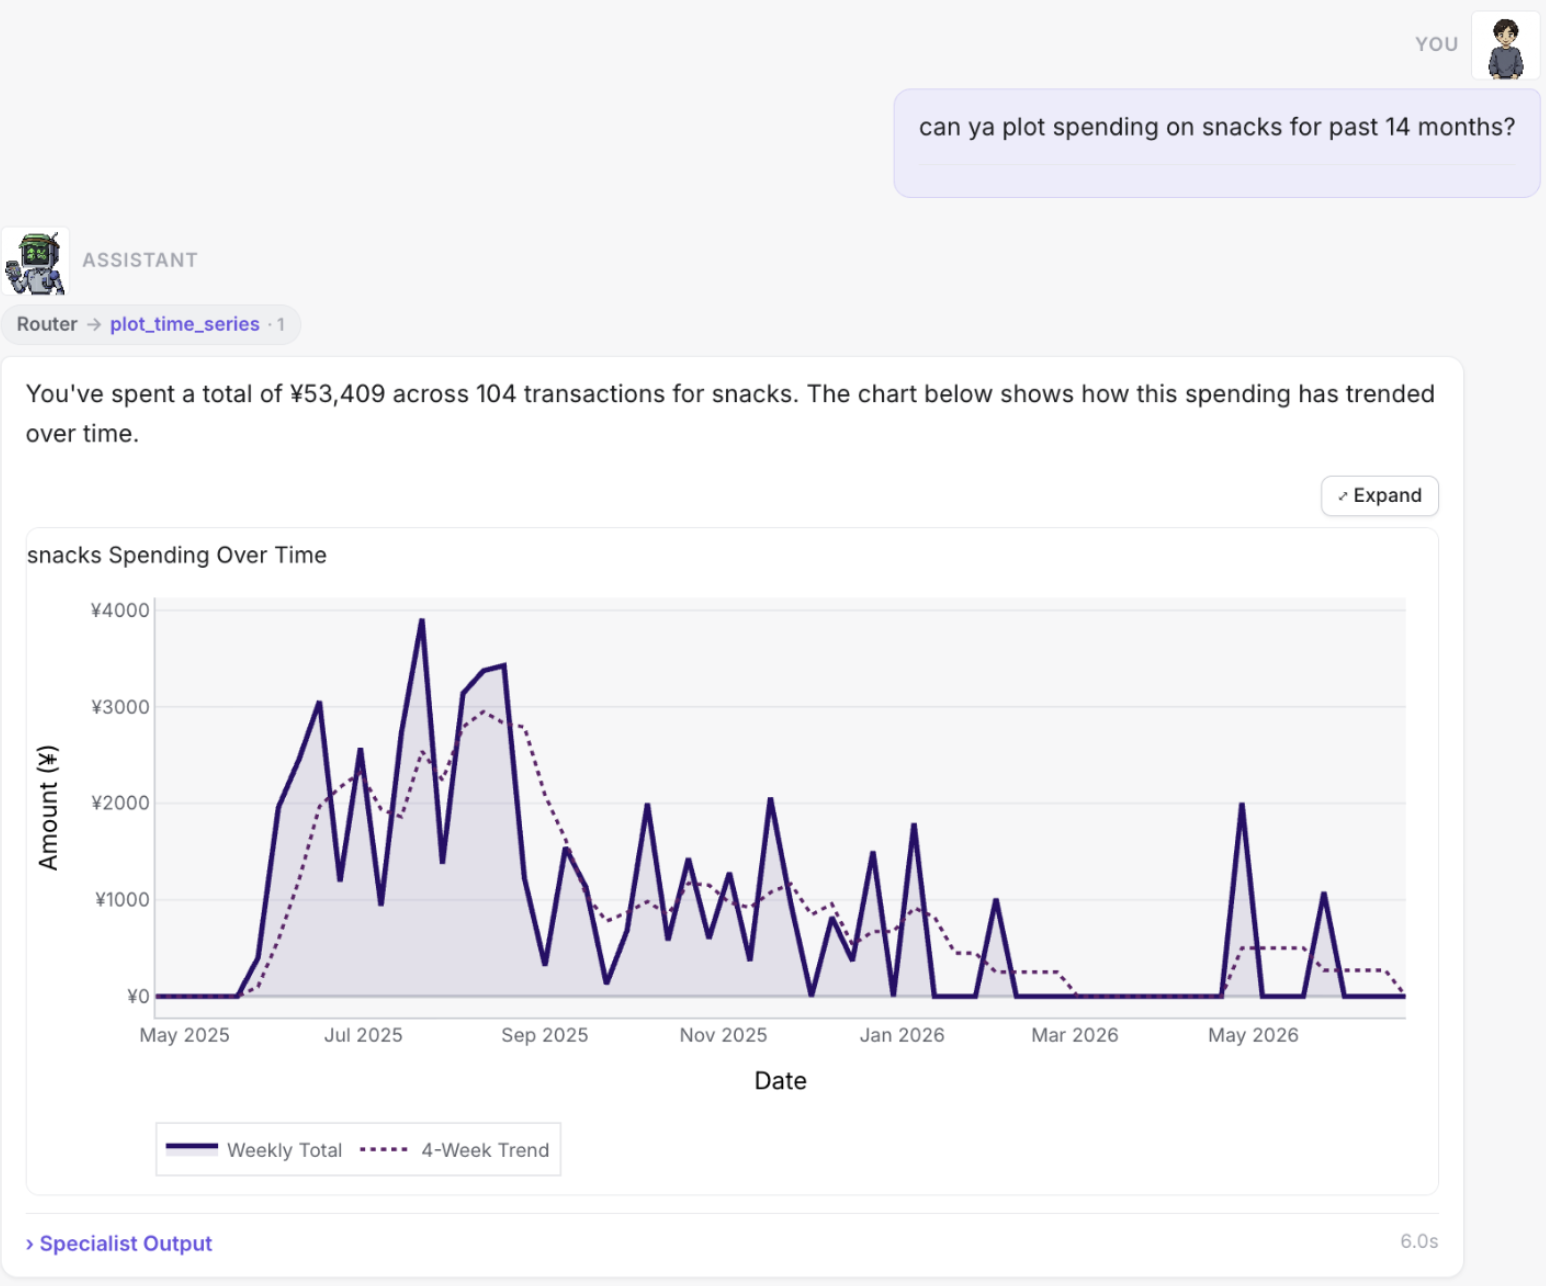
\includegraphics[width=0.68\textwidth]{og_case_cropped.png}
  \caption{Real usage session: a user queries snack spending trends
  in informal language. The dual-agent Qwen3.5-0.8B pipeline
  correctly invokes \texttt{plot\_time\_series}, producing an
  actionable spending trend---entirely on-device with no data
  transmitted externally.}
  \label{fig:case_study}
\end{figure*}

\subsection{Complexity Tier Analysis}

Figure~\ref{fig:difficulty_plot} presents the per-model accuracy
breakdown across complexity tiers in dual mode.
Task Accuracy decreases from 96\% (L1) to 82\% (L3) for
Qwen3.5-2B, and from 95\% to 84\% for Qwen3.5-0.8B.
L3 queries involve constructs like cross-year range comparisons
(\emph{``compare groceries nov 2024 to april 2025 vs nov 2025 to april 2026''}), 
which require extracting up to 10 parameters with complex
temporal constraints.


\subsection{Error Taxonomy Analysis}

Figure~\ref{fig:error_plot} visualises the full error distribution.
The error distribution shifts significantly between configurations
(\textbf{RQ3}).

For Qwen3.5-2B: single-agent produces 22.6\% \texttt{PARAM\_EXTRA}
and 7.3\% \texttt{PARAM\_MISSING}; dual-agent reduces
\texttt{PARAM\_EXTRA} to 1.9\% while \texttt{PARAM\_MISSING} remains
at 8.0\%.

The human-facing implications of this shift are significant.
A \texttt{PARAM\_EXTRA} error is a silent corruption: when a model
adds a spurious \texttt{months=1} filter to the query ``how much did I
spend on food?'', the system returns an answer- last month's food
spending- that looks correct but answers a different question.
A user relying on this figure for tax preparation, expense reporting,
or budgeting receives a plausible but wrong number, with no indication
that the scope was silently restricted.
In contrast, a \texttt{PARAM\_MISSING} error produces a visibly
broader result (e.g., all-time food spending when a month was
intended), which is more likely to trigger user scrutiny.
The dual-agent architecture's shift from extra-parameter to
missing-parameter failures thus represents a qualitative
improvement in user-facing safety, not just a numerical accuracy
improvement.

For Qwen3.5-0.8B: single-agent produces 32.5\%
\texttt{PARAM\_MISSING} and 11.8\% \texttt{PARAM\_EXTRA}; dual-agent
reduces these to 12.9\% and 11.1\% respectively, shifting the model
from a high-variance to a more predictable failure profile.

\subsection{Token Efficiency}

Figure~\ref{fig:token_efficiency} shows that despite using
$\approx$2,700 prompt tokens per query (vs.\ $\approx$5,500 for
single-agent), the dual-agent architecture achieves equivalent or
superior accuracy.
The single-agent pipeline gets access to larger contexts but exhibits lower
performance per token since the model must simultaneously attend to
all five tool schemas and disambiguation instructions.
The dual-agent architecture decomposes the context, focusing each pass
on a single subtask to achieve higher accuracy-per-token.


\subsection{Validation Layer Impact}

\begin{table}[t]
\centering
\small
\begin{tabular}{@{}lcc@{}}
\toprule
\textbf{Model (Dual)} &
$\boldsymbol{\Delta}$\textbf{Task Acc} &
$\boldsymbol{\Delta}$\textbf{CR} \\
\midrule
EXAONE-4.0     & +0.00 & +0.00 \\
Gemma-3-1B-it  & +0.12 & +0.00 \\
LFM2.5-1.2B    & +0.50 & +0.00 \\
MiniCPM5-1B    & +1.17 & +0.87 \\
Qwen3.5-0.8B   & +0.41 & +1.57 \\
Qwen3.5-2B     & +0.29 & +0.87 \\
\bottomrule
\end{tabular}
\caption{Validation layer impact ($\Delta$ in percentage points, dual
mode). Gains are modest but consistent for capable models.}
\label{tab:validation}
\end{table}

The validation layer (Table~\ref{tab:validation}) contributes modest
gains, primarily correcting category casing and normalisation.
This reveals that argument extraction remains the primary bottleneck,
since validation cannot recover missing parameters (\texttt{PARAM\_MISSING}).

% ─────────────────────────────────────────────────────────────────────────────
\vspace{-5pt}
\section{Discussion}
\label{sec:discussion}
\vspace{-3pt}
% ─────────────────────────────────────────────────────────────────────────────

\paragraph{Privacy through Task Decomposition.}
The dual-agent architecture improves accuracy and makes local
inference viable.
By separating routing (single-digit output) from extraction (focused
JSON), the dual-agent setup reduces the generation complexity per
call, addressing the primary bottleneck of small models.
Decomposing the task helps sub-2B models perform reliably on
domain-specific schemas and by doing so, makes on-device inference
a practical privacy guarantee rather than an aspirational one.

\paragraph{Metric-Specific Trade-offs.}
We note that the dual-agent advantage is not uniform across metrics.
Optimised single-agent Qwen3.5-2B achieves the highest Task Accuracy
(92.0\% vs.\ 90.4\% dual), because its joint prompt gives the model
access to all tool schemas simultaneously, enabling cross-tool
reasoning.
However, this advantage comes at a cost: single-agent produces
22.6\% \texttt{PARAM\_EXTRA} errors (vs.\ 1.9\% dual), which are
silent corruptions in financial contexts.
The dual-agent architecture is therefore preferred not because it
uniformly outperforms single-agent, but because it delivers
higher \emph{strict} correctness (Correct Ratio: 77.6\% vs.\ 60.2\%),
safer error modes, and substantially lower latency (6.2~s vs.\ 12.0~s
for Qwen3.5-2B)---properties that matter more for user-facing
financial applications.

\paragraph{Router vs.\ Simpler Intent Classifiers.}
To validate the LLM-based router, we benchmarked a lightweight
embedding-similarity baseline using
\texttt{all-MiniLM-L6-v2} (23M parameters).
Cosine similarity between query embeddings and tool-description
embeddings achieves 75.7\% tool-selection accuracy (87/115),
compared with $\geq$90\% for the LLM router across all Qwen3.5
configurations.
The embedding baseline's errors concentrate on
\texttt{plot\_time\_series} (52.2\% per-tool accuracy),
which it systematically confuses with
\texttt{plot\_comparison\_bars} when queries mention date ranges---a
contextual disambiguation task (``from 2024 to 2025'' denotes a
\emph{range} for time series, not a \emph{comparison} of two
periods) that requires pragmatic reasoning beyond lexical overlap.
Accuracy also degrades with query complexity (L1: 83.3\%,
L2: 75.6\%, L3: 71.7\%), confirming that an LLM-based router is
warranted for our domain.

\paragraph{Absence of Cloud LLM Baselines.}
We omit cloud-hosted baselines (GPT-4, Claude) because transmitting expense categories in the prompt would expose user spending patterns to third parties, violating our privacy model. Synthetic-schema cloud comparisons to quantify privacy--accuracy trade-offs are left for future work.

\paragraph{Addressing Highly Complex Queries.}
Even the best model only achieves 59.6\% strict Correct Ratio on L3
queries in dual mode, which involves complex cross-year range comparisons
requiring up to 10 interdependent parameters.
Fine-tuning on domain-specific examples using verified synthetic data
\citep{liu2024apigen} could be a potential method to improve performance on
complex queries.

\paragraph{Deployment Recommendations.}
Based on our evaluation, we recommend:
\textbf{(1)} \emph{Memory-constrained} ($\leq$2\,GB available):
Qwen3.5-0.8B dual, 89.1\% Task Acc, 3.0~s, 1.2\,GB RAM.
\textbf{(2)} \emph{Accuracy-first}: Qwen3.5-2B dual, 90.4\% Task
Acc, 77.6\% CR, 6.2~s, 2.1\,GB RAM.
\textbf{(3)} \emph{Budget hardware}: MiniCPM5-1B dual, 74.3\% Task
Acc, 43.5\% CR, 3.9~s, 1.5\,GB RAM.
All configurations keep user data entirely on-device.

\paragraph{Case Study.}
Figure~\ref{fig:case_study} shows an authentic usage session of ExpenseSense.
As a real-world deployment test in February 2026, an author used the system to query their own personal finance data in informal language-``can ya plot spending
on snacks for past X months?''. The dual-agent Qwen3.5-0.8B
pipeline correctly routed this to \texttt{plot\_time\_series} and extracted
the parameters \texttt{\{category: snacks, months: 14\}} - all in 6 seconds.
As shown in the plot, the resulting visualization revealed a clear trend in weekly
snack expenditure. By surfacing this data locally, the author was able to reflect on their habits and successfully reduce their spending over time (from peaks of \textyen3,000--4,000 to under
\textyen1,000). Crucially, this entire interaction- query, inference, and
plotting - remained strictly on the user's device; no sensitive data was transmitted
externally at any point. Connecting technical mechanisms to human needs, this demonstrates how private, local analytics can directly support personal budgeting workflows.

\vspace{-5pt}
\section{Conclusion}
\label{sec:conclusion}
\vspace{-3pt}
% ─────────────────────────────────────────────────────────────────────────────

We presented ExpenseSense, a human-centered evaluation of
privacy-preserving, on-device financial tool calling using sub-2B
quantized models.
Our central finding is that local inference at this scale is not just
technically feasible but practically reliable: Qwen3.5-0.8B in dual
mode achieves 89.1\% Task Accuracy with 3.0~s latency, keeping all
user data---queries, context, and results---strictly on-device.
Architectural decomposition into intent routing and parameter
extraction further improves strict correctness (from 60.2\% to 77.6\%
Correct Ratio)---though single-agent Qwen3.5-2B retains a slight
Task Accuracy edge (92.0\% vs.\ 90.4\%)---and, critically, shifts
error modes toward safer failures: spurious parameter additions,
which can silently corrupt financial analytics and mislead user
decisions, are replaced by missing-parameter errors that are more
visible and less harmful.

Several directions warrant future investigation:
(1) \emph{Fine-tuning} on domain-specific function-calling data to address residual L3 failures.
(2) Extending to \emph{multi-turn} interactions with conversational context.
(3) Conducting \emph{user studies} on trust and mental models of on-device privacy.
(4) Adding \emph{multilingual} query support.
(5) Evaluating generalisability to other \emph{privacy-sensitive domains} (e.g., healthcare, legal).
(6) Controlled comparisons against cloud LLMs using synthetic schemas to quantify privacy--accuracy trade-offs.
(7) Testing lower-bit quantization (Q4\_K\_M) for mobile deployment.

\vspace{-5pt}
\section*{Limitations \& Ethics}
\vspace{-3pt}
% ─────────────────────────────────────────────────────────────────────────────

\begin{itemize}\itemsep=0pt \parskip=0pt \parsep=0pt
    \item Quantisation is fixed at Q8\_0; lower-bit formats (Q4\_K\_M) may yield different tradeoffs.
    \item Test cases were single-developer authored in English; crowdsourcing and multilingual data would improve diversity.
    \item Ground-truth labels are deterministic; some queries admit alternative valid tool calls.
    \item Privacy is architectural (no external data flow) rather than cryptographic.
    \item Cloud LLMs were not benchmarked as cloud transmission violates the privacy model; evaluation is also limited to five tools in personal finance.
\end{itemize}

\vspace{-2pt}
% ─────────────────────────────────────────────────────────────────────────────
\section*{Ethics Statement}
% ─────────────────────────────────────────────────────────────────────────────

ExpenseSense is designed for on-device inference specifically to
preserve user financial privacy.
No real user financial data was used in the benchmark; all test cases
reference synthetic expense categories.
The system is intended to complement, not replace, professional
financial advice.
We recognise that even on-device models may produce incorrect
financial summaries, and advocate for clear user-facing disclaimers in
production deployments.

\vspace{-6pt}
% ─────────────────────────────────────────────────────────────────────────────
\section*{Data and Code Availability}
\vspace{-3pt}
% ─────────────────────────────────────────────────────────────────────────────

Code, prompts, benchmark data, and full results will be released on
GitHub upon acceptance.
Released artefacts include: all 115 test cases with ground-truth
labels, the complete router and specialist prompt templates, inference
configuration details, raw and validated CSV result files, and the
benchmark runner, plotting scripts, and the exact model GGUFs used in
this study to ensure complete reproducibility.

\vspace{-2pt}
\begin{small}
\setlength{\bibsep}{0pt}
\bibliography{custom}
\end{small}

% ─────────────────────────────────────────────────────────────────────────────
\appendix\onecolumn
% ─────────────────────────────────────────────────────────────────────────────

\section{Complexity Scoring Features}
\label{sec:complexity_appendix}

\begin{table}[h]
\centering
\small
\begin{tabular}{@{}llp{4.5cm}@{}}
\toprule
\textbf{Feature} & \textbf{Range} & \textbf{Description} \\
\midrule
$n_p$              & $0{+}$    & Number of expected parameters \\
$d_{\text{date}}$  & $0{-}4$   & Date complexity: none / year / month / range / specific day \\
$d_{\text{cat}}$   & $0{-}2$   & Category distance: exact / alias / semantic \\
$d_{\text{rel}}$   & $0{-}1$   & Relative time expression (``past X months'') \\
$d_{\text{multi}}$ & $0{-}2$   & Compound parameter groups \\
$d_{\text{abbr}}$  & $0{-}1$   & Abbreviated year formats (``'24'') \\
$d_{\text{hol}}$   & $0{-}2$   & Holiday/calendar knowledge required \\
\bottomrule
\end{tabular}
\caption{Seven features of the complexity scoring function
(Eq.~\ref{eq:complexity}).}
\label{tab:complexity_features}
\end{table}

\section{Known Category Vocabulary}
\label{sec:category_vocabulary}

The post-hoc parameter validation layer (Section~\ref{sec:validation}) and the LLM prompts rely on a known category vocabulary defined dynamically or in static schema files. Table~\ref{tab:categories} lists the 11 major categories defined in the application alongside the mapped subcategories/aliases from the system configuration (\texttt{categories.json}) that are passed in the \texttt{\{metadata\}} block.

\begin{table}[h]
\centering
\small
\resizebox{\textwidth}{!}{%
\begin{tabular}{@{}lp{11.5cm}@{}}
\toprule
\textbf{Major Category} & \textbf{Mapped Minor Categories / Subcategories} \\
\midrule
Housing and Utilities   & housing, internet bill, electricity bill, gas bill, water \& sewage bill, phone bill \\
Food                    & grocery, snacks, cafe, caf\'{e}, coffee, bento, beverage, combini meal, dining, eating with friend \\
Transportation          & commute, ride share, tokyo metro, Tokyo Metro, flight tickets, cable car, bus, shinkansen, car rental, taxi \\
Accommodation           & stay \\
Fitness                 & supplements, shoes, sports event, sports watch, sports clothing, sports rental, gym, sports equipment, basketball game, football game, futsal game \\
Souvenirs/Gifts/Treats  & souvenirs, treat, gift, souvenirs/gifts/treats \\
Household and Clothing  & clothing, household \\
Entertainment           & entertainment, nomikai, activities, Activities, arcades \& karaoke, Arcades \& Karaoke, events \& venues, Events \& Venues \\
Miscellaneous           & medicines, personal care, misc, help, charity, donation, entrance fees, park entrance fees, healthcare \\
Education               & tuition, books, exam fees, notebooks, textbook \\
Electronics and Furniture & furniture, electronics \\
\bottomrule
\end{tabular}%
}
\caption{Known category vocabulary from \texttt{categories.json}.}
\label{tab:categories}
\end{table}

\section{Sample Test Cases}
\label{sec:sample_tc}

\begin{table}[!ht]
\centering
\small
\resizebox{\textwidth}{!}{%
\begin{tabular}{@{}p{0.8cm}p{5.0cm}p{4.0cm}p{5.0cm}p{0.7cm}@{}}
\toprule
\textbf{ID} & \textbf{Query} & \textbf{Tool} &
\textbf{Expected Params} & \textbf{Tier} \\
\midrule
TS01 & Can ya show spending on food for past 6 months? &
\texttt{plot\_time\_series} & category=Food, months=6 & L2 \\
DI06 & show breakdown of expenses for june 21 2024 &
\texttt{plot\_distribution} & year=2024, month=6, day=21 & L2 \\
CP24 & compare groceries nov 2024 to apr 2025 vs nov 2025 to apr 2026 &
\texttt{plot\_comparison\_bars} &
category=grocery, y1=2024, sm1=11,\newline
ey1=2025, em1=4, y2=2025, sm2=11, ey2=2026, em2=4 & L3 \\
CT07 & sum total spent on metro for july 2024? &
\texttt{calculate\_total} & category=tokyo metro, year=2024, month=7 & L2 \\
TP06 & top 5 expenses past month? disregard rent &
\texttt{get\_top\_expenses} & n=5, months=1, ignore\_rent=true & L2 \\
\bottomrule
\end{tabular}%
}
\caption{Sample test cases. Note informal language, abbreviations,
and semantic mappings (``metro''$\to$``tokyo metro'',
``groceries''$\to$``grocery'').}
\label{tab:sample_tc}
\end{table}

\section{Qualitative Error Examples}
\label{sec:error_examples}

Table~\ref{tab:error_examples} illustrates representative failures
for the dominant error types in Qwen3.5-2B (dual mode).

\begin{table}[!ht]
\centering
\small
\resizebox{\textwidth}{!}{%
\begin{tabular}{@{}l p{5.0cm} p{2.5cm} p{5.5cm}@{}}
\toprule
\textbf{Error Type} & \textbf{Query} & \textbf{Expected} &
\textbf{Model Output} \\
\midrule
PARAM\_MISSING &
``Show spending trend for the last 3 months'' &
\{months: 3\} &
\{\} --- \texttt{months} omitted in the relative-time case \\[3pt]
PARAM\_VALUE\_WRONG &
``compare groceries nov 2024 to apr 2025 vs nov 2025 to apr 2026'' &
\{em1: 4, em2: 4\} &
\{em1: 11, em2: 11\} --- confuses start month for end month in
cross-year range \\[3pt]
PARAM\_EXTRA &
``How much did I spend on food?'' &
\{category: Food\} &
\{category: Food, months: 1\} --- spurious time filter restricts
scope to last month, silently returning an incorrect total \\
\bottomrule
\end{tabular}%
}
\caption{Representative failure cases for Qwen3.5-2B (dual mode).
\texttt{PARAM\_EXTRA} is the most dangerous failure mode in
financial contexts: the spurious \texttt{months=1} filter silently
restricts ``total food spending'' to ``last month's food spending'',
returning a plausible but incorrect figure that a user may act on
without realising the scope was changed.}
\label{tab:error_examples}
\end{table}

\clearpage
\section{Supplementary Figures}
\label{sec:supplementary_figures}

Figure~\ref{fig:dual_confusion_matrix} provides the routing confusion matrix across tools, while Figure~\ref{fig:combined_model_radar_grid} shows the per-category footprint across all evaluated models. Figure~\ref{fig:validation_delta_heatmap} illustrates the metrics improvement provided by the post-hoc validation layer.

\begin{figure}[htbp]
  \centering
  
\includegraphics[width=0.7\textwidth]{dual_confusion_matrix.png}
  \caption{Normalized routing confusion matrix for the dual-agent router. The moderately high diagonal accuracy (76--90\%) validates that the sequential classification step introduces negligible routing error propagation.}
  \label{fig:dual_confusion_matrix}
\end{figure}

\begin{figure}[htbp]
  \centering
  
\includegraphics[width=\textwidth]{combined_model_radar_grid.png}
  \caption{Per-model task footprint across all five task categories (Single vs. Dual mode). The dual-agent architecture provides near-universal improvement across models and tasks.}
  \label{fig:combined_model_radar_grid}
\end{figure}

\begin{figure}[htbp]
  \centering
  
\includegraphics[width=0.6\textwidth]{validation_delta_heatmap.png}
  \caption{Validation $\Delta$ Heatmap, showing absolute percentage point improvement across metrics after applying post-hoc fuzzy matching.}
  \label{fig:validation_delta_heatmap}
\end{figure}

\clearpage
\section{Prompt Templates}
\label{sec:prompts}

The on-device prompts utilized for routing and parameter extraction tasks are detailed below.

\subsection{Router Prompt}
\label{sec:router_prompt}
The router receives a focused intent-classification prompt:
\begin{scriptsize}
\begin{verbatim}
You are an expert intent classifier for an expense analysis assistant.
Your job is to determine which ONE tool is best suited to answer the user's
question.

## Available Tools

1. **`plot_time_series`** (ID: 1)
   - Use when user asks about: trends, spending over time, "past X months",
     "since 2023", date ranges.
   - Keywords: trend, over time, plot, show spending, changed, since.
   - NOTE: if user says "trend" or "over time" WITH "exclude rent", still
     use this tool.

2. **`plot_distribution`** (ID: 2)
   - Use when user asks for: breakdown, distribution, proportions, pie
     chart, "how is X split", "what does X look like".
   - Keywords: breakdown, distribution, distro, pie chart, split, look like.
   - NOTE: if user says "breakdown" or "split" WITH "exclude rent", still
     use this tool.

3. **`plot_comparison_bars`** (ID: 3)
   - Use ONLY when comparing TWO different time periods (e.g. "Dec 2024 vs
     Dec 2025" or ranges like "Jan-Jun 2024 vs Jan-Jun 2025").
   - REQUIRES two distinct periods. If the user only mentions one month or
     one year, DO NOT use this tool.
   - Keywords: compare, contrast, vs, versus, difference between.

4. **`calculate_total`** (ID: 4)
   - Use when user asks for: simple totals, sums, specific amounts "how
     much did I spend".
   - Keywords: how much, total, sum, cost.

5. **`get_top_expenses`** (ID: 5)
   - Use when user asks for: biggest/largest expenses, top X items, most
     expensive.
   - Keywords: biggest, largest, top, most expensive, highest.
   - NOTE: if user says "top X" WITH "exclude rent", still use this tool.

## Output Format
Output ONLY the tool number (1-5). Do not output anything else, NO
MARKDOWN, NO BACKTICKS, NO EXPLANATION, NO CODE!

## WRONG outputs (NEVER do this):
[X] I think the best tool is 4
[X] `4`
[X] Based on the query, I would use 1 because...
[X] ```4```
[X] The answer is: 2

## CORRECT outputs:
[v] 4
[v] 1

## Examples
User: "How much did I spend on food?"
Output: 4

User: "Total cost of internet for the last 3 months"
Output: 4

User: "How much did I spend in the last 6 months without rent?"
Output: 4

User: "Show me my spending trend for groceries"
Output: 1

User: "How has my rent changed over the last 6 months?"
Output: 1

User: "Show spending trend for past 4 months exclude rent tho"
Output: 1

User: "Compare food spending in 2024 and 2025"
Output: 3

User: "Difference in spending between Dec 2023 and Dec 2024"
Output: 3

User: "Compare overall spend in '24 vs '25 (exclude rent tho)"
Output: 3

User: "Compare dining between Jan-Jun 2024 and Jan-Jun 2025"
Output: 3

User: "Contrast spending from Nov 2024 to Feb 2025 vs Nov 2025 to Feb 2026"
Output: 3

User: "What were my biggest expenses?"
Output: 5

User: "Show me my top 5 largest purchases this year"
Output: 5

User: "Top 10 items without rent"
Output: 5

User: "Pie chart of transportation"
Output: 2

User: "How is my spending split in 2023?"
Output: 2

User: "Show me my spending breakdown excluding rent for the past 6 months"
Output: 2

User: "what does my electronics spending look like for jan 2025?"
Output: 2

User: "share distro of household expenses"
Output: 2
\end{verbatim}
\end{scriptsize}

\subsection{Specialist Base Template}
\label{sec:specialist_base}
Each specialist prompt instantiates a shared template defining output structure and relative date handling. The \texttt{\{metadata\}} placeholder is populated dynamically with the categories present in the user-uploaded dataset:
\begin{scriptsize}
\begin{verbatim}
You are an automated API parameter extractor. Your ONLY purpose is to extract
parameters from the user's request and output a SINGLE JSON object containing
those parameters.

## CRITICAL RULES (READ CAREFULLY)
1. DO NOT write any Python code or function calls. DO NOT import anything.
2. DO NOT wrap the output in markdown. NO backticks (```).
3. Output EXACTLY and ONLY a JSON object representing the parameters.
   E.g. {"category": "Food", "months": 6}
4. Use EXACT category names from the metadata below. If not an exact match,
   map it to the closest valid category (e.g. 'groceries' -> 'grocery',
   'dining out' -> 'dining').

## Date Rules
- `months=N`: RELATIVE duration (e.g. "past month" -> months=1, "last 3
  months" -> months=3, "past year" -> months=12).
- Fractional years: convert to months. "past 0.5 years" -> months=6, "past
  2.5 years" -> months=30.
- Abbreviated years: '24 = 2024, 24 = 2024, ALWAYS output the full 4-digit
  year.
- `year=YYYY`: specific full calendar year.
- `year=YYYY, month=M`: specific calendar month (e.g. "Jan 2024").
- `year=YYYY, month=M, day=D`: specific calendar date.
- `start_year=YYYY, end_year=YYYY`: specific year range.
- `start_year=YYYY, start_month=M, end_year=YYYY, end_month=M`: specific
  month-to-month range.
- For comparing two ranges (e.g., comparing Jan-Jun 2024 vs Jan-Jun 2025),
  use comparison range parameters: `y1=2024, sm1=1, em1=6, y2=2025, sm2=1,
  em2=6`.
- For comparing cross-year ranges (e.g., Nov 2024-Jan 2025 vs Nov 2025-Jan
  2026), use `ey1` and `ey2`: `y1=2024, sm1=11, ey1=2025, em1=1, y2=2025,
  sm2=11, ey2=2026, em2=1`.
- CRITICAL: For relative queries like "past month", "last month", "last 6
  months", ALWAYS use `months=N`. Do NOT use `month=M`.
- Pick ONLY ONE time filter. Do not mix `months` with `year`.

## Available Parameters
{parameters}

## Examples
{examples}

## Context
```
{metadata}
```
Currency: JPY
Today: {current_date}

FINAL REMINDER: Output ONLY the JSON object. NO MARKDOWN, NO BACKTICKS,
NO EXPLANATION, NO CODE!
\end{verbatim}
\end{scriptsize}

\subsection{Specialist Tool Prompts}
\label{sec:tool_prompts_appendix}
Each tool-specific specialist appends its unique parameter definitions and few-shot examples to the base template. The precise specifications for each tool are detailed below.

\subsubsection{plot\_time\_series}
\begin{scriptsize}
\begin{verbatim}
Parameters:
  category (str, optional), year (int, optional), month (int, optional),
  start_year (int, optional), start_month (int, optional),
  end_year (int, optional), end_month (int, optional),
  months (int, optional), ignore_rent (bool, optional, defaults to false)

## Examples
Q: "How much did I spend on futsal for the past 6 months?"
{"category": "futsal game", "months": 6}

Q: "Show me food spending from 2023 to 2025"
{"category": "Food", "start_year": 2023, "end_year": 2025}

Q: "Plot spending on snacks from oct 2024 to dec 2025"
{"category": "snacks", "start_year": 2024, "start_month": 10, "end_year": 2025, "end_month": 12}

Q: "Can ya plot spending on futsal on dec 2024?"
{"category": "futsal game", "year": 2024, "month": 12}

Q: "Gym expenses in 2024?"
{"category": "gym", "year": 2024}

Q: "Show me my spending trend for the last 3 months"
{"months": 3}

Q: "plot spending from june 2023 to dec 2025"
{"start_year": 2023, "start_month": 6, "end_year": 2025, "end_month": 12}

Q: "Trend of electricity bills since 2022"
{"category": "electricity bill", "start_year": 2022}

Q: "How has my transportation spending changed over time?"
{"category": "Transportation"}

Q: "Show spending on combinis for past year"
{"category": "combini meal", "months": 12}

Q: "Show spending trend for past 4 months exclude rent tho"
{"months": 4, "ignore_rent": true}

Q: "plot spend on cafes for past 2.5 yrs"
{"category": "cafe", "months": 30}

Q: "show my ride share costs from '24 to 26"
{"category": "ride share", "start_year": 2024, "end_year": 2026}

Q: "show electronics spending since 2023"
{"category": "electronics", "start_year": 2023}
\end{verbatim}
\end{scriptsize}

\subsubsection{plot\_distribution}
\begin{scriptsize}
\begin{verbatim}
Parameters:
  category (str, optional), year (int, optional), month (int, optional),
  day (int, optional), start_year (int, optional), start_month (int, optional),
  end_year (int, optional), end_month (int, optional), months (int, optional),
  ignore_rent (bool, optional, defaults to false)

## Examples
Q: "Show me a breakdown of my food expenses in 2024"
{"category": "Food", "year": 2024}

Q: "Pie chart of all expenses from Nov 2024 to Feb 2025"
{"start_year": 2024, "start_month": 11, "end_year": 2025, "end_month": 2}

Q: "Show me my spending breakdown for last month"
{"months": 1}

Q: "Show me my spending breakdown for groceries for past 6 months"
{"category": "Grocery", "months": 6}

Q: "show spend distribution for 2026 feb"
{"year": 2026, "month": 2}

Q: "show breakdown of all expenses from 2024 to 2025"
{"start_year": 2024, "end_year": 2025}

Q: "Show me a breakdown of expenses for Dec 2024 (exclude rent tho)"
{"year": 2024, "month": 12, "ignore_rent": true}

Q: "Show spending breakdown for 2023/06/22"
{"year": 2023, "month": 6, "day": 22}

Q: "Spending distribution for the last 3 months"
{"months": 3}

Q: "Breakdown of transportation spending from 2022 to 2024"
{"category": "Transportation", "start_year": 2022, "end_year": 2024}

Q: "How did I split my money between categories in 2023?"
{"year": 2023}

Q: "Show me my spending breakdown excluding rent for the past 6 months"
{"months": 6, "ignore_rent": true}

Q: "Breakdown of fitness spending for 2025"
{"category": "Fitness", "year": 2025}

Q: "Breakdown of my spending since 2024"
{"start_year": 2024}

Q: "show breakdown of all expenses for mar 2026 (exclude rent tho)"
{"year": 2026, "month": 3, "ignore_rent": true}

Q: "what does my electronics and furniture spending look like for jan 2025?"
{"category": "Electronics and Furniture", "year": 2025, "month": 1}
\end{verbatim}
\end{scriptsize}

\subsubsection{plot\_comparison\_bars}
\begin{scriptsize}
\begin{verbatim}
Parameters:
  category (str, optional), y1 (int, optional), m1 (int, optional),
  d1 (int, optional), y2 (int, optional), m2 (int, optional),
  d2 (int, optional), sm1 (int, optional), em1 (int, optional),
  sm2 (int, optional), em2 (int, optional), ey1 (int, optional),
  ey2 (int, optional), ignore_rent (bool, optional, defaults to false)

## Examples
Q: "Compare food spending in 2024 vs 2025"
{"category": "Food", "y1": 2024, "y2": 2025}

Q: "Compare dining Jan 2024 vs Jan 2025"
{"category": "dining", "y1": 2024, "m1": 1, "y2": 2025, "m2": 1}

Q: "How does my spend on snacks compare between jan 2024 and jan 2026?"
{"category": "snacks", "y1": 2024, "m1": 1, "y2": 2026, "m2": 1}

Q: "Compare total spending 2022 vs 2023"
{"y1": 2022, "y2": 2023}

Q: "Compare overall expenses from jan 2025 vs jan 2026"
{"y1": 2025, "m1": 1, "y2": 2026, "m2": 1}

Q: "Compare transportation on 21 July 2024 vs 21 July 2025"
{"category": "Transportation", "y1": 2024, "m1": 7, "d1": 21, "y2": 2025, "m2": 7, "d2": 21}

Q: "Compare spend on electricity 2024 vs 2025"
{"category": "electricity bill", "y1": 2024, "y2": 2025}

Q: "Compare gym spending Nov 2024 vs Nov 2025"
{"category": "gym", "y1": 2024, "m1": 11, "y2": 2025, "m2": 11}

Q: "Compare my spending in 2024 vs 2025 excluding rent"
{"y1": 2024, "y2": 2025, "ignore_rent": true}

Q: "compare education expenses '24 vs '25"
{"category": "Education", "y1": 2024, "y2": 2025}

Q: "compare household expenses for april '24 vs apr 2025"
{"category": "household", "y1": 2024, "m1": 4, "y2": 2025, "m2": 4}

Q: "Compare dining between Jan-Jun 2024 and Jan-Jun 2025"
{"category": "dining", "y1": 2024, "sm1": 1, "em1": 6, "y2": 2025, "sm2": 1, "em2": 6}

Q: "compare electricity from jan-mar '24 vs jan-mar '25"
{"category": "electricity bill", "y1": 2024, "sm1": 1, "em1": 3, "y2": 2025, "sm2": 1, "em2": 3}

Q: "Contrast overall spend from Nov 2024 to Feb 2025 vs Nov 2025 to Feb 2026"
{"y1": 2024, "sm1": 11, "ey1": 2025, "em1": 2, "y2": 2025, "sm2": 11, "ey2": 2026, "em2": 2}

Q: "compare total spend on new years eve 2024 vs for same day on 2025"
{"y1": 2024, "m1": 12, "d1": 31, "y2": 2025, "m2": 12, "d2": 31}
\end{verbatim}
\end{scriptsize}

\subsubsection{calculate\_total}
\begin{scriptsize}
\begin{verbatim}
Parameters:
  category (str, optional), year (int, optional), month (int, optional),
  day (int, optional), start_year (int, optional), start_month (int, optional),
  end_year (int, optional), end_month (int, optional), months (int, optional),
  ignore_rent (bool, optional, defaults to false)

## Examples
Q: "How much did I spend on groceries in Dec 2024?"
{"category": "grocery", "year": 2024, "month": 12}

Q: "Total spending from Oct 2024 to March 2025"
{"start_year": 2024, "start_month": 10, "end_year": 2025, "end_month": 3}

Q: "What is my total spending in 2025?"
{"year": 2025}

Q: "How much did I spend on food in past month?"
{"category": "Food", "months": 1}

Q: "Total cost of electricity in 2023"
{"category": "electricity bill", "year": 2023}

Q: "Total spent on 15 Jan 2024?"
{"year": 2024, "month": 1, "day": 15}

Q: "How much spent on rent in the last 6 months?"
{"category": "rent", "months": 6}

Q: "Sum of all transportation expenses in 2025"
{"category": "Transportation", "year": 2025}

Q: "Total spent on combini food for 2025?"
{"category": "combini meal", "year": 2025}

Q: "How much did I spend in the last 6 months without rent?"
{"months": 6, "ignore_rent": true}

Q: "Total spent on dining since 2024"
{"category": "dining", "start_year": 2024}

Q: "whats the total spend on donations from '23 to 2026?"
{"category": "donation", "start_year": 2023, "end_year": 2026}

Q: "Excluding rent, what was my total spend in 2025?"
{"year": 2025, "ignore_rent": true}
\end{verbatim}
\end{scriptsize}

\subsubsection{get\_top\_expenses}
\begin{scriptsize}
\begin{verbatim}
Parameters:
  n (int, optional, defaults to 10), category (str, optional),
  year (int, optional), month (int, optional), day (int, optional),
  start_year (int, optional), start_month (int, optional),
  end_year (int, optional), end_month (int, optional),
  months (int, optional), min_amount (int, optional),
  ignore_rent (bool, optional, defaults to false)

## Examples
Q: "What were my biggest expenses in Dec 2024?"
{"n": 10, "year": 2024, "month": 12}

Q: "Top 5 food expenses in 2024?"
{"n": 5, "category": "Food", "year": 2024}

Q: "Top 10 food expenses in june 2025?"
{"n": 10, "category": "Food", "year": 2025, "month": 6}

Q: "Top 5 expenses for 26 june 2024?"
{"n": 5, "year": 2024, "month": 6, "day": 26}

Q: "Top expenses from July 2023 to Dec 2024"
{"start_year": 2023, "start_month": 7, "end_year": 2024, "end_month": 12}

Q: "Show my top 10 expenses from 2023 to 2025"
{"n": 10, "start_year": 2023, "end_year": 2025}

Q: "Top 10 expenses of past month?"
{"n": 10, "months": 1}

Q: "What are my top expenses excluding rent?"
{"n": 10, "ignore_rent": true}

Q: "Show my top 3 largest transactions in 2023"
{"n": 3, "year": 2023}

Q: "What were the biggest expenses over the last 3 months, without rent?"
{"n": 10, "months": 3, "ignore_rent": true}

Q: "Top 7 futsal expenses for 2025?"
{"n": 7, "category": "futsal game", "year": 2025}

Q: "Top 5 expenses last month, exclude rent"
{"n": 5, "months": 1, "ignore_rent": true}

Q: "What were my biggest expenses since 2023?"
{"n": 10, "start_year": 2023}

Q: "show me top 10 expenses from jan 2025 to june '25"
{"n": 10, "start_year": 2025, "start_month": 1, "end_year": 2025, "end_month": 6}

Q: "tell me the top 15 expenses for 2025, ignore rent plz"
{"n": 15, "year": 2025, "ignore_rent": true}
\end{verbatim}
\end{scriptsize}

\end{document}